\chapter{Introdução}

\section{Motivação}
\label{sec:Motivação}

Problemas em grafos servem para modelar uma série de aplicações do dia a dia,
e há uma vasta e clássica literatura que aborda vários problemas centrais em grafos.
Estes problemas clássicos geralmente consideram um modelo estático da situação. Ou seja, o grafo dado a priori não sofre alterações enquanto estamos resolvendo o problema.

Há no entanto aplicações em que o grafo modela uma situação menos estática. Por exemplo, em redes de dispositivos de internet das coisas, chuvas, ventos fortes ou falha na fonte de energia podem prejudicar a conexão entre dispositivos, o que pode ser representado pela remoção de uma aresta no grafo que abstrai a rede.

\defi{Algoritmos em grafos dinâmicos} é o termo usado para se referir à área de projeto de algoritmos que se concentra em resolver problemas clássicos de forma eficiente nesse contexto em que o grafo está sofrendo alterações. A literatura nessa área tem mais de $40$ anos e muito progresso significativo tem ocorrido recentemente. No entanto, há uma carência de material escrito $-$ especialmente em português $-$ nos livros de algoritmos sobre essa área tão atraente e atual.

Formalmente, um \defi[grafo!dinâmico]{grafo dinâmico} de ordem~$n$ é uma sequência de grafos~$(G_0, G_1,\ldots, G_T)$, onde~$G_0$ é um grafo com $n$ vértices e
cada $G_t$ para $1\leq t\leq T$ é obtido a partir de $G_{t-1}$ pela adição ou remoção de uma aresta.
Ou seja,~$E(G_t) := E(G_{t-1})\cup \{uv\}$, para alguma aresta~$uv\notin E(G_{t-1})$;
ou $E(G_t) := E(G_{t-1})\setminus \{uv\}$, onde~$uv\in E(G_{t-1})$, respectivamente.
As operações de adição e remoção de arestas são chamadas de \defi{modificações} ou \defi{atualizações} do grafo dinâmico.

Há aplicações em que as conexões possuem um custo ou peso associado,
representando a latência de comunicação entre dispositivos ou o custo de construção de uma infraestrutura cabeada, por exemplo. 
Para lidar com tais aplicações, associa-se um valor real a cada aresta do grafo.
Nesse caso, o grafo resultante é chamado de \defi[grafo!ponderado]{ponderado}.
Em um problema com grafos dinâmicos ponderados também é considerada a operação
de mudança de peso de uma determinada aresta como uma operação de atualização válida.

Um problema em grafos dinâmicos envolve verificar se o grafo corrente~$G_t$ satisfaz alguma determinada propriedade.
A operação de verificação dessa propriedade é chamada de \defi{consulta}.
Solucionar um tal problema envolve desenvolver um algoritmo ou estrutura de dados capaz de dar suporte às modificações e consultas de forma \nolbreaks{eficiente}.

Em alguns casos, restringimos cada~$G_t$ a uma família de grafos, como, por exemplo, florestas ou~\defi[grafo!plano]{grafos planos}, isto é, um grafo que é planar, com uma imersão específica \nolbreaks{no plano}.

Trabalhar com essas classes mais restritas de grafos permite o desenvolvimento de algoritmos mais simples que podem servir de etapa intermediária para se obter uma solução para o problema geral ou ser de interesse para alguma aplicação específica.
Usaremos a primeira estratégia no estudo do nosso primeiro problema:
O \defi[problema!de conexidade em!grafos dinâmicos]{problema de conexidade em grafos dinâmicos}, que consiste em, dado um grafo dinâmico submetido a uma sequência de inserções e remoções de arestas, responder a consultas do tipo “Os vértices $u$ e $v$ estão conectados por um caminho?”.

Vamos primeiro tratar o caso em que o grafo dinâmico é uma floresta, isto é, trabalharemos com o \defi[problema!de conexidade em!florestas dinâmicas]{problema de conexidade em florestas dinâmicas},
para em seguida usar as estruturas de dados desenvolvidas nesse problema para solucionar o caso geral.

O segundo problema estudado também será restrito a uma classe específica de grafos.
Estudaremos o \defi[problema!da floresta maximal de peso mínimo em grafos ponderados dinâmicos]{problema da floresta maximal de peso mínimo em grafos ponderados dinâmicos} restrito a grafos planos.
Esse problema visa manter uma \defi{floresta maximal de peso mínimo} (MSF) de um grafo dinâmico plano ponderado ao longo de uma sequência de inserções e remoções de arestas e de modificações nos pesos das arestas.

Começaremos esse estudo na próxima seção, em que faremos uma revisão histórica dos resultados relacionados aos problemas que serão abordados nos próximos capítulos.
No Capítulo~\ref{sec:connDF}, estudaremos o problema de conexidade em florestas dinâmicas e uma de suas soluções, proposta por Holm, de Lichtenberg e Thorup~\cite{poly_log}, que envolve Euler tour trees.
Como pode ser visto no diagrama da Figura~\ref{fig:roadmap}, essa estrutura de dados utiliza treaps implícitas, que são árvores binárias de busca de chave implícita, cuja implementação será elaborada no Capítulo~\ref{sec:TreapDeChaveImplicita}.
No Capítulo~\ref{sec:connDG}, expandiremos nosso estudo sobre conexidade estudando o problema de conexidade em grafos dinâmicos.
A solução estuda também foi proposta por Holm, de Lichtenberg e Thorup~\cite{poly_log}.
Em nossos estudos, implementamos essa solução em Python3 e disponibilizamos o código no repositório git~\cite{github}.

No Capítulo~\ref{sec:MSF}, apresentaremos um algoritmo proposto por Eppstein et al.~\cite{EPPSTEIN-planar} para solucionar o problema da floresta maximal de peso mínimo em grafos dinâmicos planos ponderados.

No Capítulo~\ref{sec:lim}, mostraremos a demonstração de um limitante inferior de~$\Omega(\lg n)$ por operação para todos os problemas estudados.
Esse limitante, obtido por Patrascu e Demaine~\cite{lowerBoundPatrascu}, mostra que os algoritmos apresentados para o problema de conexidade em florestas dinâmicas e para o problema da floresta maximal de peso mínimo em grafos dinâmicos planos ponderados são assintoticamente ótimos.
No Capítulo~\ref{sec:conclusao} faremos considerações finais sobre nossos estudos.


\begin{figure}[htb]
\centering
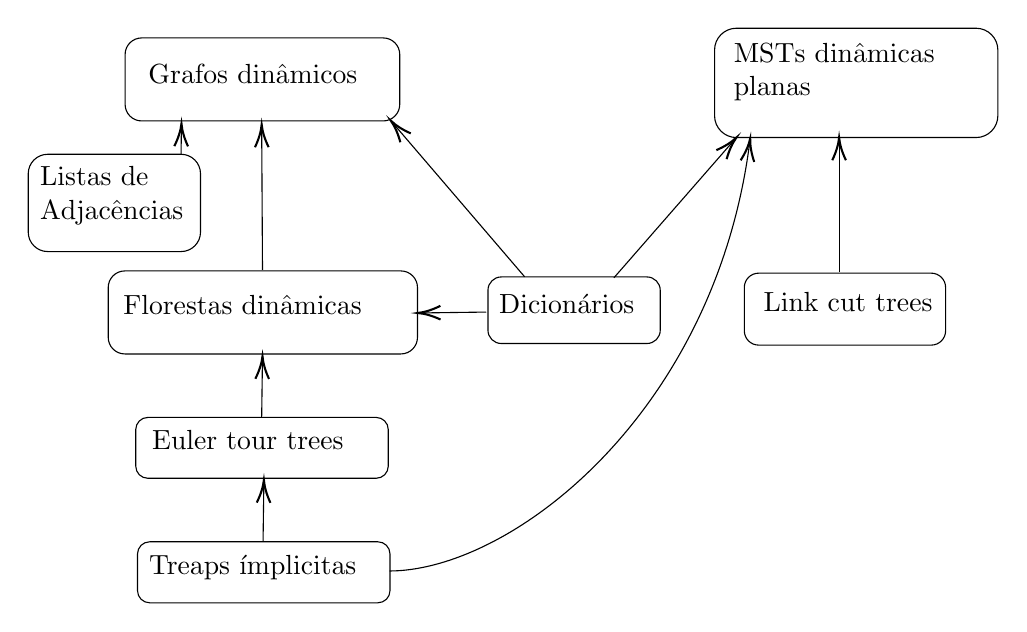
\begin{tikzpicture}[x=0.75pt,y=0.75pt,yscale=-1,xscale=1]
%uncomment if require: \path (0,390); %set diagram left start at 0, and has height of 390

%Rounded Rect [id:dp5638261819516392] 
\draw   (89.47,271.31) .. controls (89.47,268.07) and (92.1,265.43) .. (95.35,265.43) -- (205.25,265.43) .. controls (208.5,265.43) and (211.13,268.07) .. (211.13,271.31) -- (211.13,288.95) .. controls (211.13,292.2) and (208.5,294.83) .. (205.25,294.83) -- (95.35,294.83) .. controls (92.1,294.83) and (89.47,292.2) .. (89.47,288.95) -- cycle ;
%Rounded Rect [id:dp9959376432936062] 
\draw   (75.37,142.93) .. controls (75.37,138.52) and (78.95,134.93) .. (83.37,134.93) -- (216.37,134.93) .. controls (220.78,134.93) and (224.37,138.52) .. (224.37,142.93) -- (224.37,166.93) .. controls (224.37,171.35) and (220.78,174.93) .. (216.37,174.93) -- (83.37,174.93) .. controls (78.95,174.93) and (75.37,171.35) .. (75.37,166.93) -- cycle ;
%Rounded Rect [id:dp7099894103599613] 
\draw   (83.5,30.67) .. controls (83.5,26.25) and (87.08,22.67) .. (91.5,22.67) -- (207.83,22.67) .. controls (212.25,22.67) and (215.83,26.25) .. (215.83,30.67) -- (215.83,54.67) .. controls (215.83,59.08) and (212.25,62.67) .. (207.83,62.67) -- (91.5,62.67) .. controls (87.08,62.67) and (83.5,59.08) .. (83.5,54.67) -- cycle ;
%Rounded Rect [id:dp9694794812846669] 
\draw   (258.33,144.25) .. controls (258.33,140.7) and (261.2,137.83) .. (264.75,137.83) -- (334.92,137.83) .. controls (338.46,137.83) and (341.33,140.7) .. (341.33,144.25) -- (341.33,163.49) .. controls (341.33,167.03) and (338.46,169.9) .. (334.92,169.9) -- (264.75,169.9) .. controls (261.2,169.9) and (258.33,167.03) .. (258.33,163.49) -- cycle ;
%Rounded Rect [id:dp08232296692986518] 
\draw   (381.83,142.93) .. controls (381.83,139.1) and (384.94,136) .. (388.77,136) -- (471.9,136) .. controls (475.73,136) and (478.83,139.1) .. (478.83,142.93) -- (478.83,163.73) .. controls (478.83,167.56) and (475.73,170.67) .. (471.9,170.67) -- (388.77,170.67) .. controls (384.94,170.67) and (381.83,167.56) .. (381.83,163.73) -- cycle ;
%Rounded Rect [id:dp3985250366724754] 
\draw   (367.5,28.53) .. controls (367.5,22.72) and (372.22,18) .. (378.03,18) -- (493.47,18) .. controls (499.28,18) and (504,22.72) .. (504,28.53) -- (504,60.13) .. controls (504,65.95) and (499.28,70.67) .. (493.47,70.67) -- (378.03,70.67) .. controls (372.22,70.67) and (367.5,65.95) .. (367.5,60.13) -- cycle ;
%Straight Lines [id:da5589289981455373] 
\draw    (149.7,134.4) -- (149.31,66.4) ;
\draw [shift={(149.3,64.4)}, rotate = 89.67] [color={rgb, 255:red, 0; green, 0; blue, 0 }  ][line width=0.75]    (10.93,-3.29) .. controls (6.95,-1.4) and (3.31,-0.3) .. (0,0) .. controls (3.31,0.3) and (6.95,1.4) .. (10.93,3.29)   ;
%Straight Lines [id:da8087039160610074] 
\draw    (149.3,205.6) -- (149.67,178) ;
\draw [shift={(149.7,176)}, rotate = 90.77] [color={rgb, 255:red, 0; green, 0; blue, 0 }  ][line width=0.75]    (10.93,-3.29) .. controls (6.95,-1.4) and (3.31,-0.3) .. (0,0) .. controls (3.31,0.3) and (6.95,1.4) .. (10.93,3.29)   ;
%Straight Lines [id:da19920966114360028] 
\draw    (257.5,154.75) -- (226.5,155.17) ;
\draw [shift={(224.5,155.2)}, rotate = 359.22] [color={rgb, 255:red, 0; green, 0; blue, 0 }  ][line width=0.75]    (10.93,-3.29) .. controls (6.95,-1.4) and (3.31,-0.3) .. (0,0) .. controls (3.31,0.3) and (6.95,1.4) .. (10.93,3.29)   ;
%Straight Lines [id:da38139604958901885] 
\draw    (319,138.25) -- (376.72,72.17) ;
\draw [shift={(378.03,70.67)}, rotate = 131.14] [color={rgb, 255:red, 0; green, 0; blue, 0 }  ][line width=0.75]    (10.93,-3.29) .. controls (6.95,-1.4) and (3.31,-0.3) .. (0,0) .. controls (3.31,0.3) and (6.95,1.4) .. (10.93,3.29)   ;
%Straight Lines [id:da5633794503104798] 
\draw    (427.5,135.33) -- (427.5,72.67) ;
\draw [shift={(427.5,70.67)}, rotate = 90] [color={rgb, 255:red, 0; green, 0; blue, 0 }  ][line width=0.75]    (10.93,-3.29) .. controls (6.95,-1.4) and (3.31,-0.3) .. (0,0) .. controls (3.31,0.3) and (6.95,1.4) .. (10.93,3.29)   ;
%Straight Lines [id:da7918857844120134] 
\draw    (276,137.75) -- (212.8,64.02) ;
\draw [shift={(211.5,62.5)}, rotate = 49.4] [color={rgb, 255:red, 0; green, 0; blue, 0 }  ][line width=0.75]    (10.93,-3.29) .. controls (6.95,-1.4) and (3.31,-0.3) .. (0,0) .. controls (3.31,0.3) and (6.95,1.4) .. (10.93,3.29)   ;
%Rounded Rect [id:dp21131335155672382] 
\draw   (36.83,88.11) .. controls (36.83,82.93) and (41.03,78.73) .. (46.21,78.73) -- (110.46,78.73) .. controls (115.64,78.73) and (119.83,82.93) .. (119.83,88.11) -- (119.83,116.23) .. controls (119.83,121.4) and (115.64,125.6) .. (110.46,125.6) -- (46.21,125.6) .. controls (41.03,125.6) and (36.83,121.4) .. (36.83,116.23) -- cycle ;
%Straight Lines [id:da7631806191728931] 
\draw    (110.46,78.73) -- (110.63,65.93) ;
\draw [shift={(110.66,63.93)}, rotate = 90.77] [color={rgb, 255:red, 0; green, 0; blue, 0 }  ][line width=0.75]    (10.93,-3.29) .. controls (6.95,-1.4) and (3.31,-0.3) .. (0,0) .. controls (3.31,0.3) and (6.95,1.4) .. (10.93,3.29)   ;
%Curve Lines [id:da8410667922534024] 
\draw    (211,279.5) .. controls (270.37,279.17) and (367.69,202.93) .. (384.42,73.13) ;
\draw [shift={(384.67,71.17)}, rotate = 96.96] [color={rgb, 255:red, 0; green, 0; blue, 0 }  ][line width=0.75]    (10.93,-3.29) .. controls (6.95,-1.4) and (3.31,-0.3) .. (0,0) .. controls (3.31,0.3) and (6.95,1.4) .. (10.93,3.29)   ;
%Rounded Rect [id:dp3745338241823657] 
\draw   (88.63,211.37) .. controls (88.63,208.13) and (91.26,205.5) .. (94.5,205.5) -- (204.43,205.5) .. controls (207.67,205.5) and (210.3,208.13) .. (210.3,211.37) -- (210.3,228.97) .. controls (210.3,232.21) and (207.67,234.83) .. (204.43,234.83) -- (94.5,234.83) .. controls (91.26,234.83) and (88.63,232.21) .. (88.63,228.97) -- cycle ;
%Straight Lines [id:da6552331155919412] 
\draw    (149.97,265.27) -- (150.34,237.67) ;
\draw [shift={(150.37,235.67)}, rotate = 90.77] [color={rgb, 255:red, 0; green, 0; blue, 0 }  ][line width=0.75]    (10.93,-3.29) .. controls (6.95,-1.4) and (3.31,-0.3) .. (0,0) .. controls (3.31,0.3) and (6.95,1.4) .. (10.93,3.29)   ;

% Text Node
\draw (93.8,270.43) node [anchor=north west][inner sep=0.75pt]   [align=left] {Treaps ímplicitas};
% Text Node
\draw (81.37,145.6) node [anchor=north west][inner sep=0.75pt]   [align=left] {Florestas dinâmicas};
% Text Node
\draw (93.5,34.33) node [anchor=north west][inner sep=0.75pt]   [align=left] {Grafos dinâmicos};
% Text Node
\draw (262.5,145) node [anchor=north west][inner sep=0.75pt]   [align=left] {Dicionários};
% Text Node
\draw (389.83,144) node [anchor=north west][inner sep=0.75pt]   [align=left] {Link cut trees};
% Text Node
\draw (375.5,24) node [anchor=north west][inner sep=0.75pt]   [align=left] {MSTs dinâmicas\\planas};
% Text Node
\draw (41.3,83.4) node [anchor=north west][inner sep=0.75pt]   [align=left] {Listas de\\Adjacências};
% Text Node
\draw (95.3,210.5) node [anchor=north west][inner sep=0.75pt]   [align=left] {Euler tour trees};
\end{tikzpicture}

\caption{Diagrama com estruturas de dados usadas. Uma seta de A para B significa que a estrutura de dados B usa a estrutura de dados A.}
\label{fig:roadmap}
\end{figure}

\section{Historiografia}

Essa seção é inspirada na historiografia apresentada em \cite{HHSRecentAdvances2022, Zaroliagis2002}.

Soluções para os problemas de conexidade dinâmica e de floresta maximal de peso mínimo se desenvolveram em paralelo ao longo dos anos. Em $1975$, Spira e Pan~\cite{SP1975} atacaram o problema MSF propondo um algoritmo cuja complexidade é $\O{n}$ para inserção e $\O{n^2}$ para remoção de arestas, onde $n$ é o número de vértices do grafo. Três anos depois, Chin e Houck~\cite{CH1978} apresentaram uma solução mais simples para inserção e remoção de arestas que possui o mesmo consumo de tempo que o algoritmo de Spira e Pan.

Em $1985$, Frederickson~\cite{frederickson1983data} reduziu a complexidade de ambas as operações de modificação para $\O{\!\sqrt{m}}$, onde~$m$ é o número de arestas do grafo no momento em que a operação é aplicada.
Em $1992$, Eppstein et al.~\cite{Eppstein1992SparsificationaTF,Eppstein1997SparsificationaTF} melhoraram o consumo de tempo do algoritmo de Frederickson para~$\O{\!\sqrt{n}}$.

O primeiro algoritmo poli-logarítmico para o problema de conectividade dinâmica foi apresentado por Henzinger e King~\cite{HenzingerKing} em~$1995$ e possui consumo amortizado esperado $\O{\lg^3 n}$ para cada operação. Nesse artigo, elas propuseram a utilização de uma estrutura de dados chamada Euler tour trees como uma maneira eficiente de representar florestas dinâmicas.
Em seguida, em $1997$, o consumo amortizado esperado por operação foi reduzido a $\O{\lg^2 n}$~\cite{HenzingerThorup} e, nesse mesmo ano, foi realizado o primeiro estudo experimental, avaliando diferentes versões do algoritmo de Frederickson~\cite{xpAnalyGiuseppe}.

Ainda em~$1995$, Nikoletseas, Reif, Spirakis e Yung~\cite{NikoletseasRSY} propuseram uma estrutura de dados para o problema \defi[grafo!estocástico]{estocástico} de conexidade em grafos dinâmicos, em que a sequência de atualizações e consultas é escolhida ao acaso com probabilidade uniforme.
Nessas condições, essa estrutura de dados permite fazer atualizações em tempo~$\O{\lg^3 n}$ esperado amortizado e consulta em tempo~$\O{1}$ esperado amortizado.

Em $1999$, Fatourou, Spirakis, Zarafidis, e Zoura~\cite{Fatourou} implementaram os algoritmos de Henzinger e King~\cite{HenzingerKing} e de Nikoletseas et al.~\cite{NikoletseasRSY} e os compararam experimentalmente.
Eles concluíram que a estrutura de dados de Nikoletseas et al. tem uma performance melhor do que a de Henzinger e King quando o grafo dinâmico estocástico é denso.

Inspirados na solução de Henzinger e King para o problema de conexidade dinâmica, em $1998$, Holm, de Lichtenberg e Thorup~\cite{poly_log} atacaram ambos os problemas de conectividade dinâmica e de MSF usando Euler tour trees.
A solução deles para o problema de conexidade empata com o consumo assintótico da solução de Henzinger e King de~$\O{\lg^2 n}$.
No entanto, se a implementação das Euler tour trees for determinística, então o algoritmo para conexidade dinâmica de Holm et al. é completamente determinístico e seu consumo é somente amortizado,
enquanto que o consumo na solução de Henzinger e King é esperado e amortizado. 
Apresentaremos a solução de Holm et al. nesse texto com uma implementação aleatorizada de Euler tour trees.
Avaliações experimentais foram feitas sobre essa solução~\cite{EmpiricalStudy1997, EmpiricalStudy2002,xp-Phylogeny}.
Comentaremos esses experimentos no Capítulo~\ref{sec:conclusao}.

O algoritmo de Holm et al. para MSF possui consumo amortizado $\O{\lg^4 n}$ para cada operação, sendo assim a primeira estrutura de dados determinística com consumo de tempo poli-logarítmico para o problema MSF. Uma implementação eficiente deste algoritmo foi apresentada por Cattaneo et al. \cite{xpstudy2002} junto a um outro algoritmo mais simples e assintoticamente pior, mas que teve bom desempenho nos experimentos práticos realizados.

Em $2000$, Thorup~\cite{Thorup2000} complementou o algoritmo de Holm et al.~\cite{poly_log}, adicionando uma estrutura de dados auxiliar chamada floresta estrutural, que reduz o consumo de tempo de cada operação para~$\O{\lg n\, (\lg\lg n)^3}$ esperado amortizado e~$\O{\frac{\lg n}{\lg \lg \lg n}}$ para a consulta de conexidade.
Ela só não é ótima por um fator de $\O{(\lg\lg n)^3}$, devido ao limitante inferior de~$\Omega(\lg n)$ provado em~$2006$ por Patrascu e Demaine~\cite{lowerBoundPatrascu}.

Em $2010$, Tarjan e Werneck~\cite{tarjanWerneck2010} fizeram um estudo experimental com diversas estruturas de dados para árvores dinâmicas que resolvem ambos os problemas de conexidade em florestas dinâmicas e da floresta maximal de peso mínimo,
destacando qualidades e deficiências de cada estrutura de dados quando sujeitas a diferentes tipos de cargas de trabalho. 

Desde $1997$, os algoritmos com consumo de tempo amortizado foram predominantes na literatura, porém todos possuem alguma instância com consumo de tempo $\OTheta{n}$ no pior caso.
O problema de melhorar o tempo assintótico no pior caso continuou a permear a literatura sem avanços até $2013$, quando Kapron, King e Mountjoy \cite{bruceM} apresentaram uma estrutura de dados para o problema de conexidade em grafos dinâmicos baseada no problema \textit{cutset} que proporciona consumo $\O{\lg^4 n}$ para a inserção de arestas, $\O{\lg^5 n}$ para remoção e responde à consulta de conexidade em tempo~$\O{\frac{\lg n}{\lg\lg n}}$.
A estrutura responde a consultas corretamente quando a resposta é “sim” e com alta probabilidade de acerto quando a resposta é “não”. A probabilidade de falso positivo, mesmo que baixa, continuou incentivando a pesquisa na área. 

\newpage
Em $2015$, Kejlberg-Rasmussen et al.~\cite{kejlbergrasmussen_et_al} apresentaram uma estrutura de dados para o problema de conexidade em grafos dinâmicos que permite fazer consultas em tempo constante, mas que possui consumo de tempo para as atualizações de~$\mathrm{O}\!\left(\sqrt{\frac{n\left(\lg \lg n\right)^2}{\lg n}}\right)$, um consumo de tempo assintótico consideravelmente maior do que os últimos algoritmos citados.

Em $2016$, Wulff-Nilsen~\cite{Wulff-Nilsen2016} apresentou um novo algoritmo para o problema de conexidade em grafos dinâmicos que dá suporte às atualizações com consumo~$\O{\frac{\lg^2 n}{\lg \lg n}}$ amortizado e~$\O{\frac{\lg n}{\lg \lg n}}$ para a consulta de conexidade.

Em $2017$, Huang et al.~\cite{fastestConn} reorganizam a solução de Thorup~\cite{Thorup2000} obtendo uma solução com consumo de tempo de~$\O{\lg n\, (\lg\lg n)^2}$ esperado amortizado para cada atualização e~$\O{\frac{\lg n}{\lg \lg \lg n}}$ para as consultas de conexidade.
Essa é atualmente a estrutura de dados com menor consumo de tempo assintótico conhecida para solucionar o problema de conexidade em grafos dinâmicos.

Em $2022$, Chen et al. \cite{QC22} propuseram uma heurística baseada no diâmetro do grafo dinâmico e com ela desenvolveram um algoritmo que possui bom desempenho prático quando aplicado a grafos dinâmicos extraídos de situações reais.
O consumo de tempo dessa heurística é linear em função do diâmetro do grafo, portanto as operações de atualização e de consulta possuem consumo de tempo de~$\O{n}$ no pior dos casos.
Veja um resumo dos resultados mencionados nesta seção na Tabela~\ref{tab:historiografia}
\begin{table}[h!]
\centering
\begin{tabular}{||c | c | c | c | c | c||} 
 \hline
 ano & inserção & remoção & consulta & tipo & ref. \\ [0.5ex] 
 \hline\hline
	$1985$ & $\O{\!\sqrt{m}}$ & $\O{\!\sqrt{m}}$ & $\O{1}$  & {\small determinístico; pior caso} & \cite{frederickson1983data} \\ 
 \hline
	$1992$ & $\O{\!\sqrt{n}}$ & $\O{\!\sqrt{n}}$ & $\O{1}$  & {\small determinístico; pior caso} & \cite{Eppstein1992SparsificationaTF} \\ 
 \hline
	$1995$ & $\O{\lg^3 n}$ & $\O{\lg^3 n}$   & $\O{\lg n}$  & {\small aleatorizado; amortizado} & \cite{HenzingerKing} \\ 
 \hline
	$1997$ & $\O{\lg^2 n}$ & $\O{\lg^2 n}$   & $\O{\lg n}$  & {\small aleatorizado; amortizado} & \cite{HenzingerThorup} \\ 
 \hline
	$1998$ & $\O{\lg^2 n}$ & $\O{\lg^2 n}$   & $\O{\lg n}$  & {\small determinístico; amortizado} & \cite{poly_log} \\ 
 \hline
	$2000$ & $\O{{\scriptstyle \lg n(\lg  \lg n)^3}}$ &  $\O{{\scriptstyle \lg n(\lg \lg n)^3}}$      & $\O{\frac{\lg n}{\lg\lg\lg n}}$  & {\small aleatorizado; amortizado }& \cite{Thorup2000} \\ 
 \hline
	$2013$ & $\O{\lg^4 n}$ & $\O{\lg^5 n}$ & $\O{{\scriptstyle \lg n / \lg \lg n }}$ & {\small determinístico; pior caso} & \cite{bruceM} \\
 \hline
	$2015$ & $ \mathrm{O}\!\left(\sqrt{\frac{n\left(\lg \lg n\right)^2}{\lg n}}\right)  $ & $\mathrm{O}\!\left(\sqrt{\frac{n\left(\lg \lg n\right)^2}{\lg n}}\right)$ & $\O{1}$ & {\small determinístico; pior caso} & \cite{kejlbergrasmussen_et_al} \\
 \hline
	$2016$ & $\O{  \frac{\lg^2 n}{\lg \lg n}}$ & $\O{ \frac{\lg^2 n}{\lg \lg n}} $   & $\O{ \frac{\lg n}{\lg \lg n}} $  & {\small determinístico; amortizado} & \cite{Wulff-Nilsen2016} \\ 
 \hline
	$2017$ & $\O{{\scriptstyle \lg n(\lg  \lg n)^2}}$ &  $\O{{\scriptstyle \lg n(\lg \lg n)^2}}$      & $\O{\frac{\lg n}{\lg\lg\lg n}}$  & {\small aleatorizado; amortizado }& \cite{fastestConn} \\ 
 \hline
	$2022$ & $\O{n}$ & $\O{n} $   & $\O{n} $  & {\small determinístico; pior caso } & \cite{QC22} \\ 
 \hline
\end{tabular}
\caption{Consumo de tempo de estruturas de dados para o problema de conexidade em grafos dinâmicos.}
\label{tab:historiografia}
\end{table}
